\documentclass[a4paper, 12pt]{article}

\usepackage{preamble}
\usepackage{listings}
\usepackage{graphicx}
\usepackage{amsmath}

\begin{document}
\newgeometry{left=2cm,right=2cm,top=2cm,bottom=1cm,bindingoffset=0cm}
\begin{titlepage}

    \begin{center}
        \vspace*{5cm}
        \Huge Московский Физико-Технический Институт
        \vspace*{2cm}\\
        \LARGE Отчет по эксперименту
        \\\vspace*{0.25cm}

        \noindent\rule{\textwidth}{1pt}
        \vspace*{-0.25cm}

        \huge \textbf{Низкоуровневая оптимизация параллельных алгоритмов}
        \noindent\rule{\textwidth}{1pt}


       \vfill
        \begin{flushright}
            \begin{minipage}{.4\textwidth}
            \Large Выполнил:\\ Студент 1 курса ФРКТ\\ Группа Б01-302 \\Хальфин Бахтияр\\
            \end{minipage}
        \end{flushright}

        \vfill
        \normalsize Долгопрудный \\2024

    \end{center}
\end{titlepage}
\restoregeometry



\section*{Ключевые слова}
\noindent \MakeUppercase{параллелизм, векторизация, оптимизация, SIMD, AVX, AVX2, intinsic функции, множество мандельброта, фракталы}\\

\textbf{Цель работы:} оптимизировать функцию, обрабатывающую большое количество значений, и сравнить производительность разных реализаций. В качестве оптимизируемой функции используется функция расчета множества Мандельброта. \\

\textbf{Оборудование:} Персональный компьютер (ПК) с центральным процессором (ЦП), поддерживающим как минимум AVX2 инструкции; монитор; клавиатура и мышь. \\

\textbf{Программное обеспечение:} Операционая система (ОС) Linux; компилятор GCC или Clang; графическая библиотека SDL2 с расширением SDL2\_ttf; инструмент для сборки проекта Make; программа визуализирующая множество Мандельброта\\

\textbf{Полученные результаты:} 
\begin{itemize}
    \item Флаги оптимизации компилятора g++ ускорили \textit{примитивную} реализацию в \textbf{3.06} раз, \textit{векторную} в \textbf{8.83} раза, \textit{intrinsic} в \textbf{5.88} раз
    \item Флаги оптимизации компилятора clang++ ускорили \textit{примитивную} реализацию в \textbf{3.14} раз, 
    \textit{векторную} в \textbf{24.67} раза, \textit{intrinsic} в \textbf{6.48} раз
    \item В данной задаче компилятор clang++ показал себя лучше -- он ускорил \textit{векторизированную} реализацию в \textbf{2.79} раз больше g++
    \item Реализация с \textit{intrinsic} функциями работает быстрее \textit{векторной}, но она имеет существенный недостаток в плохой переносимости.
\end{itemize}
\newpage

\section*{Введение}
\subsection*{Теоретические сведения}

\textit{Параллельные вычисления} - это тип вычислений, в котором множество вычислений или процессов выполняются одновременно. 

\textit{Векторизация (в параллельных вычислениях)} — вид распараллеливания программы, при котором однопоточные приложения, выполняющие одну операцию в каждый момент времени, модифицируются для выполнения нескольких однотипных операций одновременно.

Скалярные операции, обрабатывающие по паре операндов, заменяются на операции над векторами, обрабатывающие несколько элементов вектора в каждый момент времени.\\

Например,  фрагмент программы, который поэлементно перемножает два массива может быть векторизирован следующим образом.

\begin{figure}[!htb]
   \begin{minipage}{0.48\textwidth}
    \begin{lstlisting}
for (i = 0; i < 1024; i++)
    C[i] = A[i] * B[i];
    \end{lstlisting}
   \end{minipage}\hfill
   \begin{minipage}{0.48\textwidth}
    \begin{lstlisting}
for (i = 0; i < 1024; i+=4)
    C[i:i+3] = A[i:i+3] * B[i:i+3];
    \end{lstlisting}
   \end{minipage}
\end{figure}

Запись $C[i:i+3]$ означает вектор из 4 элементов — от $C[i]$ до $C[i+3]$ включительно, а под * понимается операция поэлементного умножения векторов. Векторный процессор в данном примере сможет выполнить 4 скалярные операции при помощи одной векторной.\\

\begin{figure}[!htb]
    \begin{minipage}{0.48\textwidth}
        \centering
        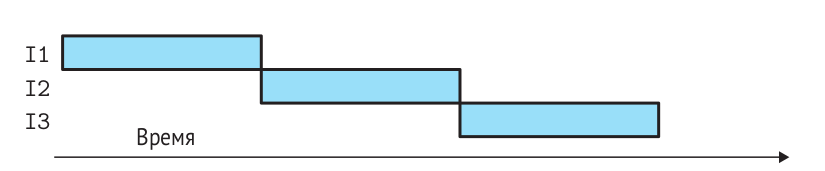
\includegraphics[width=1\linewidth]{scalar_example.png}
        \caption{Неконвейерная реализация}
    \end{minipage}\hfill
    \begin{minipage}{0.48\textwidth}
        \centering
        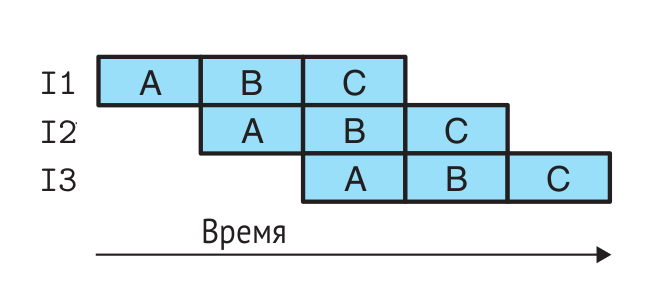
\includegraphics[width=1\linewidth]{parallel_example.png}
        \caption{Конвейерная реализация}
    \end{minipage}
\end{figure}

\textit{SIMD} (англ. single instruction, multiple data — одиночный поток команд, множественный поток данных) — принцип компьютерных вычислений, позволяющий обеспечить параллелизм на уровне данных.

Короткие SIMD инструкции (64 или 128 бит) стали появляться в 1990-х годах.
В 2010 году компания Intel представила SIMD-расширение AVX в процессорах архитектуры Sandy Bridge.

\textit{Intrinsic (англ. внутренний) функции} -  это функции, реализация которой специально обрабатывается компилятором. Как правило, она может заменять последовательность автоматически генерируемых инструкций для вызова оригинальной функции, подобно \textit{inline} функции. В отличие от \textit{inline} функции, компилятор обладает глубокими знаниями о \textit{intrinsic} функции и поэтому может лучше интегрировать и оптимизировать ее для конкретной ситуации.

\textit{Intrinsic} функции часто используются для векторизации и параллелизации. Компиляторы для C и C++ преобразуют \textit{intinsic} непосредственно в \textit{SIMD} инструкции.

\subsection*{Множество Мандельброта}
\begin{figure}[h]
    \centering
    
\includegraphics[width=1\linewidth]{mandelbrot_example.png}
    \caption{Пример визуализации множества Мандельброта}
\end{figure}
\textit{Множество Мандельброта} — множество точек c на комплексной плоскости, которое задается рекуррентным соотношением $Z_n = Z_n^2 + c$, где $Z_0 = 0$.

Иначе говоря, это множество таких $с$, для которых существует такое действительное $R$, что неравенство $|z_n| < R$ выполняется при всех натуральных n.\\

Множество Мандельброта является одним из самых известных фракталов, в том числе за пределами математики, благодаря своим цветным визуализациям
\subsubsection*{Построение множества}
Переформулируем соотношение, описанное выше. Заменим $Z_n$ на $x_n$ и $y_n$ и получим значения координат комплексной плоскости $(x, y)$:
\begin{align} 
    x_{n+1} = x_n^2 - y_n^2 + x_0 \nonumber\\
    y_{n+1} = 2x_ny_n + y_0 \label{calc_expressions}
\end{align}

Очевидно, что как только модуль $Z_n$ окажется больше 2, все последующие модули последовательности станут стремиться к бесконечности. В случае $|c| > 2$ это можно доказать с помощью метода математической индукции. При |c| > 2 точка c заведомо не принадлежит множеству Мандельброта, что можно вывести методом математической индукции, используя равенство $Z_0 = 0$.
\newpage

\section*{Виды реализаций вычислений множества Мандельброта}
\subsubsection*{Простой}
В данной реализации выражения (\ref{calc_expressions}) просто переведены в код на C, каждый пиксель обрабатывается отдельно

\begin{lstlisting}
    FOR EACH pixel on the screen (x0, y0)
        x := x0
        y := y0
    
        i := 0
        FOR i TO MAX_ITERATION_NUMBER
            IF x*x + y*y > 4 THEN
                BREAK
            END IF
    
            x = x*x - y*y + x0
            y = 2*x*y + y0
            i++
        ENDLOOP
        
        PAINT(x0, y0, i)
\end{lstlisting}

\subsubsection*{Векторный}
В данной реализации обрабатываются вектора из 8 чисел. Действие над каждым вектором происходит в цикле.\\

Приводить псвевдокод данной реализации не имеет особого смысла, так как он в точности повторяет предыдущую. 
\subsubsection*{С intrinsic функциями}
В данной реализации используются AVX2 инструкции, одновременно обрабатываются 8 пикселей.

\begin{lstlisting}
    FOR EACH 8 pixels on the screen (x0, y0)
        x := x0
        y := y0
        i := _mm256_setzero_si256();
        FOR i TO MAX_ITERATION_NUMBER
            x2      := _mm256_mul_ps(x,  x)
            y2      := _mm256_mul_ps(y,  y)
            xy      := _mm256_mul_ps(x,  y)
            radius2 := _mm256_add_ps(x2, y2)
    
            cmp_mask := _mm256_cmp_ps(radius2, MAX_RADIUS_2_256,
                                      _CMP_LT_OQ)
            IF (_mm256_testz_ps(cmp_mask, cmp_mask)) THEN
                BREAK
            END IF
    
            x = _mm256_add_ps(x0, _mm256_sub_ps(x2, y2))
            y = _mm256_add_ps(y0, _mm256_add_ps(xy, xy))
    
            iterations = _mm256_sub_epi32(iterations,
                         _mm256_castps_si256(cmp_mask))
        ENDLOOP
    
        PAINT(x0,y0, i)
\end{lstlisting}

\section*{Экспериментальная установка}
Характеристики системы, на которой снимались значения:
\begin{table}[h]
    \centering
    \begin{tabular}{|c|c|}
        \hline
        OS         & Linux Mint 21.3 x86\_64 \\\hline
        Kernel     & 6.1.0-1036-oem          \\\hline
        CPU        & AMD Ryzen 7 5700U       \\\hline
    \end{tabular}
\end{table}


\section*{Методика измерений}
\begin{table}[h]
    \centering
    \begin{tabular}{|c|c|}
        \hline
        Разрешение           & 1600x900 \\\hline
        Количество вызовов   & 100      \\\hline
        Макс. Число итераций & 256      \\\hline
        Координаты по X      & 0        \\\hline
        Координаты по Y      & 0        \\\hline
        Значение Zoom        & 1        \\\hline
    \end{tabular}
    \caption{Параметры программы}
\end{table}
Вычисляется разница тактов перед многократным вызовом функции и после.
Количество тактов вычисляется с помощью функции clock() из библиотеки time.h.\\

Измерения проводятся для версии программы скомпилированной с помощью компиляторов GCC и Clang с различными флагами компиляции\\

С целью увеличить точность полученных значений, ограничим количество ядер, на которых работает система. Таким образом, влияние остальных процессов на наши измерения будут значительно сокращено. Также это позволяет улучшить кэширование.

В файле /etc/systemd/system.conf установим значение переменной CPUAffinity на 0-2. После перезагрузки системы все процессы будут выполняться на первых трех ядрах.
Будем запускать программу через комманду taskset -c 14 ./mandelbrot. Так наша программа будет выполняться на ядре с номером 14.\\

Измерение на каждой конфигурации будем проводить по два раза. Первый результат будем отбрасывать, он необходим для \textit{прогрева кэша}.


\section*{Результаты измерений}
В следующих двух таблицах П*, В*, И* означают простая реализация, векторная реализация и реализация с \textit{Intrinsic} функциями соответсвенно.\\

\begin{table}[h]
    \begin{tabular}{|l|l|l|l|l|l|}
    \hline
        g++ & -O0 & -O1 & -O2 & -O3 & -Ofast \\ \hline
        П* & 8336413 & 3070945 & 3117255 & 3116930 & 2724064 \\ \hline
        В* & 15741537 & 4981874 & 5418236 & 1914521 & 1782368 \\ \hline
        И* & 2730567 & 503628 & 514620 & 513366 & 464273 \\ \hline
        П* (такты / вызов) & 83364,13 & 30709,45 & 31172,55 & 31169,30 & 27240,64 \\ \hline
        В* (такты / вызов) & 157415,37 & 49818,74 & 54182,36 & 19145,21 & 17823,68 \\ \hline
        И* (такты / вызов) & 27305,67 & 5036,28 & 5146,20 & 5133,66 & 4642,73 \\ \hline
        П* (кадры / с) & 12,00 & 32,56 & 32,08 & 32,08 & 36,71 \\ \hline
        В* (кадры / с) & 6,35 & 20,07 & 18,46 & 52,23 & 56,11 \\ \hline
        И* (кадры / с) & 36,62 & 198,56 & 194,32 & 194,79 & 215,39 \\ \hline
        П*/В* & 0,53 & 0,62 & 0,58 & 1,63 & 1,53 \\ \hline
        П*/И* & 3,05 & 6,10 & 6,06 & 6,07 & 5,87 \\ \hline
        В*/И* & 5,76 & 9,89 & 10,53 & 3,73 & 3,84 \\ \hline
    \end{tabular}
    \caption{Количество тактов для каждой конфигурации}
\end{table}

\begin{table}[h]
\begin{tabular}{|l|l|l|l|l|l|}
    \hline
       Clang++ & -O0 & -O1 & -O2 & -O3 & -Ofast \\ \hline
        П* & 8404013 & 3141622 & 3053549 & 3055993 & 2671065 \\ \hline
        В* & 14989553 & 5047541 & 639773 & 639767 & 607709 \\ \hline
        И* & 2958196 & 540116 & 503991 & 502373 & 456579 \\ \hline
        П* (такты / вызов) & 84040,13 & 31416,22 & 30535,49 & 30559,93 & 26710,65 \\ \hline
        В* (такты / вызов) & 149895,53 & 50475,41 & 6397,73 & 6397,67 & 6077,09 \\ \hline
        И* (такты / вызов) & 29581,96 & 5401,16 & 5039,91 & 5023,73 & 4565,79 \\ \hline
        П* (кадры / с) & 11,90 & 31,83 & 32,75 & 32,72 & 37,44 \\ \hline
        В* (кадры / с) & 6,67 & 19,81 & 156,31 & 156,31 & 164,55 \\ \hline
        И* (кадры / с) & 33,80 & 185,15 & 198,42 & 199,06 & 219,02 \\ \hline
        П*/В* & 0,56 & 0,62 & 4,77 & 4,78 & 4,40 \\ \hline
        П*/И* & 2,84 & 5,82 & 6,06 & 6,08 & 5,85 \\ \hline
        В*/И* & 5,07 & 9,35 & 1,27 & 1,27 & 1,33 \\ \hline
    \end{tabular}
    \caption{Количество тактов для каждой конфигурации}
\end{table}
\newpage

\raggedright
В следующей диаграмме названия с индексом один означают компилятор g++, с индексом 2 -- clang++ 
\begin{figure}[h]
    \centering
    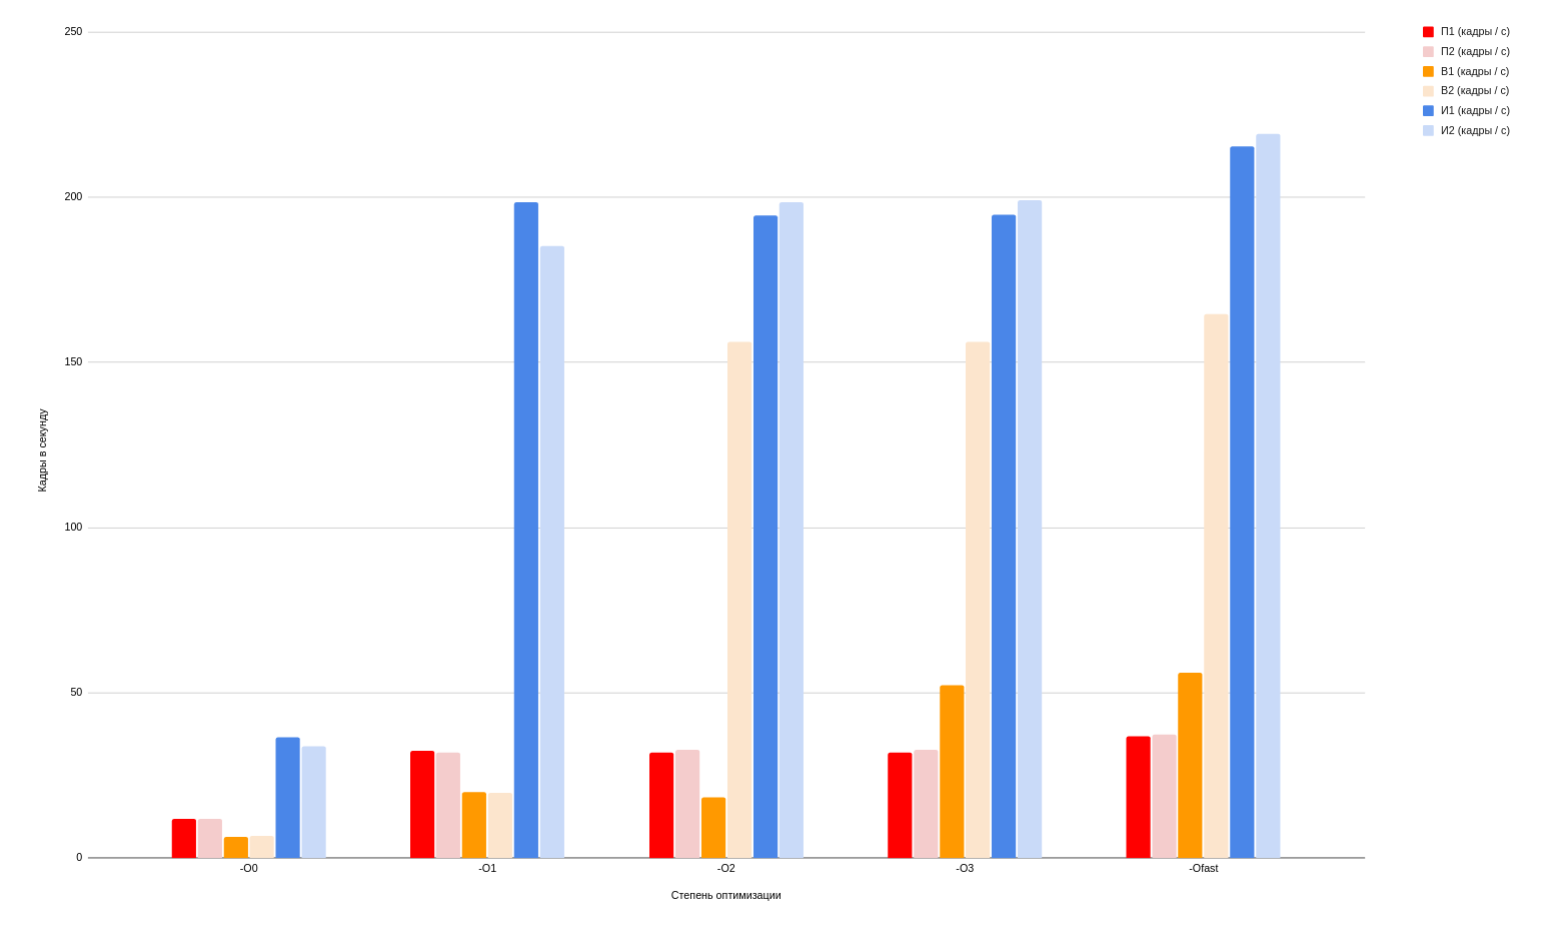
\includegraphics[width=1\linewidth]{chart.png}
    \caption{Сравнение скорости программы, скомпилированной через g++ и clang++}
\end{figure}

\raggedright
\section*{Список литературы}
\begin{enumerate}
    \item Р. Брайант, Д. О`Халларон "Компьютерные системы. Архитектура и программирование".
    \item Intrinsic function - https://en.wikipedia.org/wiki/Intrinsic\_function
    \item Mandelbrot set - https://en.wikipedia.org/wiki/Mandelbrot\_set
\end{enumerate}

\end{document}
